\section{HEDM (BraggNN)}
{{\footnotesize
\begin{description}[labelwidth=5em, labelsep=1em, leftmargin=*, align=left, itemsep=0.3em, parsep=0em]
  \item[date:] 2023-10-03
  \item[version:] TODO
  \item[last\_updated:] 2023-10
  \item[expired:] unknown
  \item[valid:] yes
  \item[valid\_date:] TODO
  \item[url:] \href{https://arxiv.org/abs/2008.08198}{https://arxiv.org/abs/2008.08198}
  \item[doi:] TODO
  \item[domain:] Material Science
  \item[focus:] Fast Bragg peak analysis using deep learning in diffraction microscopy
  \item[keywords:]
    - BraggNN
    - diffraction
    - peak finding
    - HEDM
  \item[summary:] Uses BraggNN, a deep neural network, for rapid Bragg peak localization in 
high-energy diffraction microscopy, achieving about 13x speedup compared 
to Voigt-based methods while maintaining sub-pixel accuracy.

  \item[licensing:] TODO
  \item[task\_types:]
    - Peak detection
  \item[ai\_capability\_measured:]
    - High-throughput peak localization
  \item[metrics:]
    - Localization accuracy
    - Inference time
  \item[models:]
    - BraggNN
  \item[ml\_motif:]
    - Real-time, Image/CV
  \item[type:] Framework
  \item[ml\_task:]
    - Peak finding
  \item[solutions:] TODO
  \item[notes:] Enables real-time HEDM workflows; basis for NAC case study.

  \item[contact.name:] Jason Weitz (UCSD)
  \item[contact.email:] unknown
  \item[results.links.name:] ChatGPT LLM
  \item[fair.reproducible:] True
  \item[fair.benchmark\_ready:] True
  \item[ratings.software.rating:] 0
  \item[ratings.software.reason:] Not analyzed. 

  \item[ratings.specification.rating:] 10.0
  \item[ratings.specification.reason:] Fully specified: describes task (data filtering/classification, system design (on-sensor inference), 
latency (25 ns), and power constraints.

  \item[ratings.dataset.rating:] 8.0
  \item[ratings.dataset.reason:] In-pixel charge cluster data used, but dataset release info is minimal; FAIR metadata/versioning limited.

  \item[ratings.metrics.rating:] 9.0
  \item[ratings.metrics.reason:] Data rejection rate and power per pixel are clearly defined and directly tied to hardware goals.

  \item[ratings.reference\_solution.rating:] 9.0
  \item[ratings.reference\_solution.reason:] 2-layer NN implementation is evaluated in hardware; reproducible via hls4ml flow with results in paper.

  \item[ratings.documentation.rating:] 8.0
  \item[ratings.documentation.reason:] Paper is clear; Zenodo asset is referenced, but additional GitHub or setup repo would improve reproducibility.

  \item[id:] hedm\_braggnn
  \item[Citations:] \cite{liu2021braggnnfastxraybragg}
  \item[Ratings:]
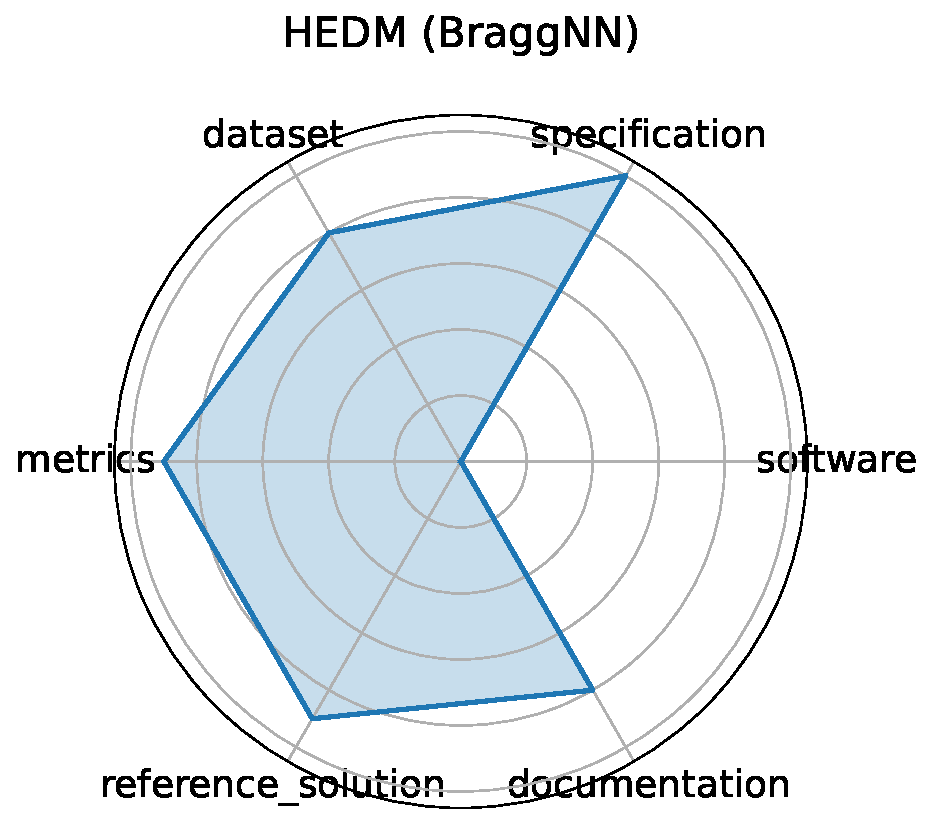
\includegraphics[width=0.2\textwidth]{hedm_braggnn_radar.pdf}
\end{description}
}}
\clearpage